% !TeX program = lualatex
\documentclass[12pt]{IEEEtran}
\IEEEoverridecommandlockouts
\usepackage{fancyhdr}
\usepackage{graphicx}
\usepackage[spanish, es-tabla, es-nodecimaldot]{babel}
\usepackage{csquotes}
\usepackage{wrapfig}
\usepackage[l3]{csvsimple}
\usepackage{array}
\usepackage[calc, spanish]{datetime2}
\usepackage{enumitem}
\usepackage{multirow}
\usepackage{mismath}
\usepackage[export]{adjustbox}
\usepackage{nccmath}
\usepackage{amsmath}
\usepackage{amssymb}
\usepackage{mathtools}
\usepackage{amsfonts,latexsym} % para tener disponibilidad de diversos simbolos
\usepackage{empheq}
\usepackage{derivative}
\usepackage{float}
\usepackage{threeparttable}
\usepackage{subcaption}
\usepackage{ifpdf}
\usepackage{rotating}
\usepackage{stfloats}
\usepackage{tabularray}
\UseTblrLibrary{siunitx}
% \usepackage[inline]{showlabels}
\usepackage{kantlipsum}
\usepackage{siunitx}
\usepackage{afterpage}
\usepackage[
  sorting=none,
  backend=biber,
  citestyle=numeric-comp,
]{biblatex}
\usepackage{hyperref}
\usepackage{cleveref}
\crefname{table}{tabla}{tablas} % Table's cross-reference name
\crefname{equation}{ec.}{ecs.} %
\newcommand\crefrangeconjunction{--}
\newcommand\crefpairconjunction{~y~}
%%%%%%%%%%%%%%%%%%%%%%%%%%%%%%%%%%%%%%%%%%%
%%% CREAR Y REESCRIBIR ALGUNOS COMANDOS %%%
%%%%%%%%%%%%%%%%%%%%%%%%%%%%%%%%%%%%%%%%%%%
\newcolumntype{P}[1]{>{\centering\arraybackslash}p{#1}}  %% Se crea un nuevo tipo de columna llamada P.
\newcommand{\ctt}{\centering\scriptsize\textbf} %%\ctt abrevia el comando \centering\scriptsize\textbf
\newcommand{\dtt}{\scriptsize\textbf} %%\dtt abrevia el comando \scriptsize\textbf
\renewcommand\IEEEkeywordsname{Palabras clave}

%%%%%%%%%%%%%%%%%%%%%%%%%%%%%%%%%%%%%%%%%%%
\graphicspath{ {figs/} {logos/}}  %%Ruta donde se encuentran las imágenes, que esté vacio indica que las imagenes están dentro de la misma carpeta que contiene el archivo .tex
\addbibresource{bibliography.bib}
\sisetup{
  output-decimal-marker = {.},
  uncertainty-mode = separate,
  separate-uncertainty-units=single,
  uncertainty-mode=separate,
}
%%%%%%%%%%%%%%%%%%%%%%%%%%%%%%%%%%%%%%%%%%%%%%%%%%%%%%%%%%
%%%%%%%%%%% ENCABEZADO DE LAS PÁGINAS TIPO FC %%%%%%%%%%%%%%%
%%%%%%%%%%%%%%%%%%%%%%%%%%%%%%%%%%%%%%%%%%%%%%%%%%%%%%%%%%

\newcommand{\MYhead}{\smash{\scriptsize
\hfil\parbox[t][\height][t]{\textwidth}{\centering
\begin{picture}(0,0) \put(-0,-15){\includegraphics[width=33mm]{LogoFC}} \end{picture} \hspace{6.5 cm}
Reporte De Práctica \hspace{5.15cm} \hphantom{Versión 1.0}\\
\hspace{6.85cm} Facultad de Ciencias Grupo 8462\hspace{4.65cm} Semestre 2026-3\\
\underline{\hspace{ \textwidth}}}\hfil\hbox{}}}
\makeatletter
% normal pages
\def\ps@headings{%
\def\@oddhead{\MYhead}%
\def\@evenhead{\MYhead}}%
% title page
\def\ps@IEEEtitlepagestyle{%
\def\@oddhead{\MYhead}%
\def\@evenhead{\MYhead}}%
\makeatother
% make changes take effect
\pagestyle{headings}
% adjust as needed
\addtolength{\footskip}{0\baselineskip}
\addtolength{\textheight}{-1\baselineskip}

%%%%%%%%%%%%%%%%%%%%%%%%%%%%%%%%
%%%%% INICIO DEL DOCUMENTO %%%%%
%%%%%%%%%%%%%%%%%%%%%%%%%%%%%%%%


\DTMsavedate{duedate}{2026-01-30}% Año-Mes-Día -> Fecha de entrega
\DTMnewdatestyle{usvardate}{%
  \renewcommand{\DTMdisplaydate}[4]{%
    \DTMMonthname{##2}\nobreakspace% Mes
    \number##1% Año
  }%
  \renewcommand{\DTMDisplaydate}{\DTMdisplaydate}%
}

\begin{document}
%%%%%%%%%%%%%%%%%%%%%%%%%%%%
%%% TÍTULO DEL DOCUMENTO %%%
%%%%%%%%%%%%%%%%%%%%%%%%%%%%

\title{Medición de la rapidez de la luz}

%%%%%%%%%%%%%%%%%%%%%%%%%%%
%%%%%%%%% AUTORES %%%%%%%%%
%%%%%%%%%%%%%%%%%%%%%%%%%%%
\author{\IEEEauthorblockN{Wei Yang Guan Montes, Marcos López Merino, \\
		Yassar Emanuel Pérez Evaristo, Victor Ramos}\\
	\IEEEauthorblockA{\textbf{Profesor}: Víctor Manuel Velázquez Aguilar}\\
	\IEEEauthorblockN{\DTMusedate{duedate}}}

%%%%%%%%%%%%%%%%%%%%%%%%%%%
\twocolumn[
	\begin{@twocolumnfalse}
		\maketitle
		\begin{abstract}
			A partir de los valores para la función de correlación de
			segundo orden \(g^{(2)}(0)\) para pares de fotones generados
			por conversión paramétrica espontánea descendente, se caracterizó
			el comportamiento clásico o cuántico de una fuente de luz mediante
			mediciones del número de coincidencias basadas en el efecto Hanbury
			Brown y Twiss.
			Para ello, se emplearon configuraciones experimentales con dos
			detectores (haz transmitido y haz reflejado) y con tres detectores,
			añadiendo uno correspondiente al haz testigo, realizando 400
			experimentos con una duración de \(\qty{1}{\s} \pm \qty{0.05}{\us}\)
			y un tiempo de coincidencia de \qty{5 \pm 0.05}{\ns}, con el fin
			de obtener una máxima anticorrelación.

		\end{abstract}

		\begin{IEEEkeywords}
			Fotones, SPDC, Hanbury Brown y Twiss, HBT, función de correlación, fuente
			cuántica
		\end{IEEEkeywords}
	\end{@twocolumnfalse}
	\vspace{1cm}
]

%%%%%%%%%%%%%%%%%%%%%%
%\IEEEpeerreviewmaketitle
%%%%%%%%%%%%%%%%%%%%%%%%%%%%%%%%%%%%%
%%% PRIMERA SECCIÓN DEL DOCUMENTO %%%
%%%%%%%%%%%%%%%%%%%%%%%%%%%%%%%%%%%%%
\section{Introducción}
\kant[1]

\section{Procedimiento experimental}
\kant[2]

\section{Resultados y análisis}

\subsection{Medición del tiempo}

En esta sección se presentan los resultados de la medición del tiempo entre las
transiciones a la mitad de altura de dos pulsos obtenidos del conteo de fotones
provenientes del láser de bombeo violeta\cite{laserBCL100405} con una longitud
de onda de \qty{405(4)}{\nm}.

A partir de los datos experimentales se construyó un histograma de los tiempos
de coincidencia (ver
\cref{fig:histograma-f1}),
el cual permite visualizar la distribución estadística de los eventos
registrados y verificar la consistencia del proceso de detección.

\begin{figure*}[htb]
	\centering
	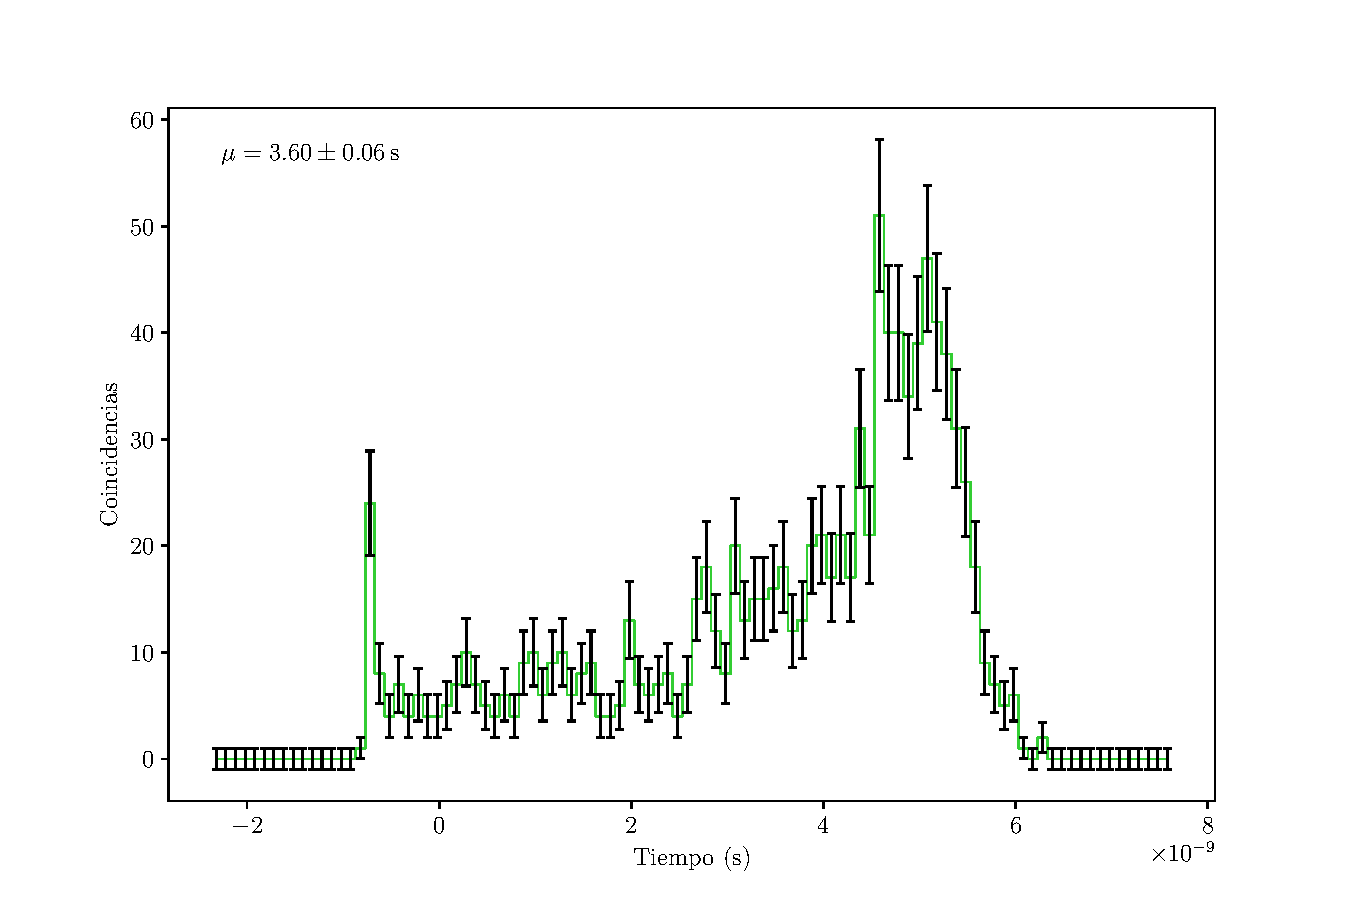
\includegraphics[width=0.8\textwidth]{figs/histogram.pdf}
	\caption{Histograma del número de coincidencias de tiempo de las señales de
		los pulsos detectados.}
	\label{fig:histograma-f1}
\end{figure*}

De esta distribución se realizó el análisis estadístico correspondiente para obtener un valor representativo del tiempo que sería utilizado para el cálculo de la rapidez de la luz. Dado que los datos provienen de un proceso de conteo de coincidencias, se asumió una estadística de Poisson para los eventos registrados. El tiempo medio se obtuvo a partir de un promedio de la distribución, mientras que la incertidumbre asociada se calculó como el error estadístico del promedio, determinado a partir de la dispersión de los datos y del número total de cuentas.

\begin{equation}
	t = \qty{3.60 \pm 0.06}{\ns}
	\label{eq:mean-time-transition-ns-e1}
\end{equation}

\subsection{Distancia entre detectores}

Para determinar la distancia entre los detectores, cada uno de los integrantes
del equipo realizó una medición independiente utilizando un flexómetro con resolución de \qty{0.1}{\cm}. Los valores obtenidos se muestran en la \cref{tblr:distance-between-detectors-t1}.

\begin{table}[htb]
	\centering
	\begin{tblr}{
			colspec = { Q[si={table-format=3.1(2),table-number-alignment=center, uncertainty-mode = separate}, c, 22mm]},
			cell{1}{1} = {r=2}{guard, mode = text, valign=m},
			hlines,
			vlines,
		}
		{ Distancia   \\
		(\unit{\cm})} \\
		\\
		135.0(0.05)   \\
		135.0(0.05)   \\
		135.8(0.05)   \\
		135.3(0.05)
	\end{tblr}
	\caption{Mediciones de la separación entre detectores realizada por cada
		integrante del equipo.}
	\label{tblr:distance-between-detectors-t1}
\end{table}

A partir de los datos de la \cref{tblr:distance-between-detectors-t1}
se obtuvo la separación promedio entre los detectores, calculada como el
promedio de las mediciones individuales. La incertidumbre asociada se determinó
considerando dos contribuciones independientes: la incertidumbre instrumental
asociada a la resolución del flexómetro y la incertidumbre estadística debida a
la dispersión entre las mediciones individuales. Ambas contribuciones se
combinaron para obtener la incertidumbre total en la distancia promedio.

\begin{equation}
	d = \qty{1.353(0.0019)}{\m}
	\label{eq:separation-detector-e2}
\end{equation}

\section{Cálculo de la rapidez de la velocidad de la luz}

El valor de la rapidez de la luz se obtuvo utilizando la relación

\begin{equation*}
	c = \dfrac{d}{t},
\end{equation*}

donde \(d\) corresponde a la separación entre los detectores y \(t\) al tiempo
medio de coincidencia medido experimentalmente. Usando los valores obtenidos en
las
\cref{eq:mean-time-transition-ns-e1,eq:separation-detector-e2},
se obtuvo que la rapidez de la luz es

\begin{equation*}
	c = \qty[per-mode=symbol]{3.75(0.07)e8}{\m\per\second}.
\end{equation*}

La incertidumbre de la rapidez de la luz se obtuvo mediante propagación de
incertidumbres, siendo la incertidumbre temporal la contribución dominante.

\section{Conclusiones}
\kant[4]

%%%%%%%%%%%%%%%%%%%%%%%%%%%%%%%%
%%%%%%    Bibliografia   %%%%%%%
%%%%%%%%%%%%%%%%%%%%%%%%%%%%%%%%
\nocite{*}
\clearpage
\printbibliography
\end{document}
